\documentclass[letter,twoside,11pt]{article}

\usepackage[spanish,es-nodecimaldot]{babel}
\usepackage[utf8]{inputenc}

\usepackage{lmodern}
\usepackage[T1]{fontenc}
\usepackage{textcomp}

\usepackage{framed}
\usepackage[svgnames]{xcolor}
\colorlet{shadecolor}{Gainsboro!50}

\usepackage[labelfont=bf]{caption}
\usepackage{graphicx}
\usepackage{pstricks}

\usepackage{anysize}
\marginsize{3cm}{2cm}{2cm}{3cm}

\usepackage{siunitx}
\usepackage{amsmath}
\usepackage{array}
\usepackage{alltt}
\usepackage{csquotes}

\usepackage{fancyhdr}
\usepackage{lastpage}
\pagestyle{fancy}
\fancyhf{}
\fancyhead[LE,RO]{Electrónica Analógica I}
\fancyfoot[CO,CE]{\thepage\ de \pageref{LastPage}}

\special{papersize=215.9mm,279.4mm}

\usepackage[
    pdfauthor={Carlos Eduardo Caballero Burgoa},%
    pdftitle={Electrónica Analógica I},%
    pdfsubject={Calculo de transistor},%
    colorlinks,%
    citecolor=black,%
    filecolor=black,%
    linkcolor=black,%
    urlcolor=black,
    breaklinks]{hyperref}
\usepackage{breakurl}

\newcommand{\blankpage}{
\newpage
\thispagestyle{empty}
\mbox{}
\newpage
}

\renewcommand{\arraystretch}{1.2}

\DeclareUnicodeCharacter{03A9}{~}

\begin{document}

\begin{titlepage}
    \begin{center}
        {\Large UNIVERSIDAD MAYOR DE SAN SIMÓN}\\
        \vspace*{0.15cm}
        {\large FACULTAD DE CIENCIAS Y TECNOLOGÍA}\\
        \vspace*{0.10cm}
        DEPARTAMENTO DE ELÉCTRICA-ELECTRÓNICA\\
        \vspace*{3.0cm}
        {\Large \textbf{ELECTRÓNICA ANALÓGICA I}}\\
        %\vspace*{0.3cm}
        %{\Large \textbf{REPORTE No. 1}}\\
        \vspace*{3.5cm}
        {\Large \textbf{TRANSISTOR JFET POLARIZADO POR \\
        MEDIO DE UN DIVISOR DE VOLTAJE}}\\
    \end{center}

    \vspace*{6.1cm}
    \leftskip=7.95cm
    \noindent
    \textbf{Estudiante:}\\
    Caballero Burgoa, Carlos Eduardo.\\
    Herbas Nava, Adrian.\\
    \newline
    \textbf{Carrera:}\\
    Ing. Electromecánica.\\
    \newline
    \textbf{Docente:}\\
    Ing. Alberto Arispe Santander.\\
    \newline
    \textbf{Grupo:} 2.\\
    \textbf{Fecha de entrega:} 12 de Noviembre del 2024.\\
\end{titlepage}
\addtocounter{page}{-1}

\blankpage
\addtocounter{page}{-1}

Este documento detalla las pruebas que se realizaron sobre un transistor
\textbf{2N3819} en un divisor de voltaje con una fuente de CD de
$9[\text{V}]$ para hallar las cuatro resistencias que manejen el mejor margen
de trabajo en la curva característica del transistor $\text{JFET}$.

\section{Introducción}
Dado el circuito de la \textbf{figura~\ref{circuito1}}, se hallan los valores de
las resistencias obtener un punto $Q$ estable.

\begin{figure}[!h]
\centering
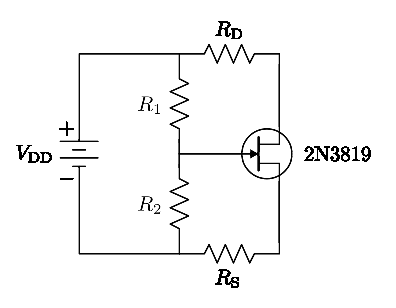
\includegraphics[scale=1.0]{figura1.eps}
\caption{Circuito de polarización con divisor de voltaje.}
\label{circuito1}
\end{figure}

Una curva de transferencia para un \textbf{JFET} se expresa aproximadamente
como:
\begin{equation*}
    I_{\text{D}} \cong I_{\text{DSS}}
    \left(1-\frac{V_{\text{GS}}}{V_{\text{GS(corte)}}}\right)^2
\end{equation*}

La recta de carga de CD con divisor de voltaje se determina de la siguiente
manera:

Con $I_\text{D} = 0$:
\begin{equation*}
    \begin{split}
        V_\text{S} &= I_{\text{D}}\,R_{\text{S}}\\
                   &= (0)\,R_{\text{S}}\\
                   &= 0[V]\\
        V_\text{GS} &= V_{\text{G}} - V_{\text{S}}\\
                    &= V_{\text{G}} - 0[V]\\
                    &= V_{\text{G}}\\
    \end{split}
\end{equation*}

Donde $V_{\text{G}}$:
\begin{equation*}
    V_{\text{G}} = \left(\frac{R_2}{R_1+R_2}\right)\,V_{\text{DD}}
\end{equation*}

Por consiguiente, un punto sobre la recta está en $I_{\text{D}} = 0$ y
$V_{\text{GS}} = V_{\text{G}}$.

Con $V_{\text{GS}} = 0$:
\begin{equation*}
    \begin{split}
        I_\text{D} &= \frac{V_{\text{G}} - V_{\text{GS}}}{R_{\text{S}}}\\
                   &= \frac{V_{\text{G}}}{R_{\text{S}}}\\
    \end{split}
\end{equation*}

El punto donde la recta de carga corta la curva de transferencia es el punto
$Q$ \cite{Floyd}.
\begin{equation*}
    \begin{split}
        \frac{1}{-R_{\text{S}}}\,(V_{\text{GS}}-V_{\text{G}}) &=
        I_{\text{DSS}}
        \left(1-\frac{V_{\text{GS}}}{V_{\text{GS(corte)}}}\right)^2\\
        \frac{V_{\text{G}}}{R_{\text{S}}}-\frac{V_{\text{GS}}}{R_{\text{S}}} &=
        I_{\text{DSS}}
        \left(1-2\frac{V_{\text{GS}}}{V_{\text{GS(corte)}}}+
        \frac{V_{\text{GS}}^2}{V_{\text{GS(corte)}}^2}\right)\\
        0 &= \left(\frac{I_{\text{DSS}}}{V_{\text{GS(corte)}}^2}\right)\,
        V_{\text{GS}}^2 + \left(\frac{1}{R_{\text{S}}}-
        \frac{2\,I_{\text{DSS}}}{V_{\text{GS(corte)}}}\right)\,
        V_{\text{GS}}+
        \left(I_{\text{DSS}}-\frac{V_{\text{G}}}{R_{\text{S}}}\right)\\
    \end{split}
\end{equation*}

Resolviendo la ecuación cuadrática es posible encontrar el punto $Q$ del
circuito.

\section{Hoja de datos}
La hoja de datos del transistor \textbf{2N3819} se detalla en el
\textbf{Cuadro~\ref{hojadedatos}} \cite{2N3819}.

\begin{table}[!h]
\begin{center}
    \begin{tabular}{|c|l|c|c|c|}
    \hline
    \multicolumn{5}{|c|}{\textbf{Valores nominales absolutos máximos}}
    \tabularnewline \hline
    \textbf{Símbolo} &
    \textbf{Parámetro} &
    \multicolumn{2}{|c|}{\textbf{Valor}} &
    \textbf{Unidades}
    \tabularnewline \hline \hline
    $V_{\text{DG}}$ &
    Voltaje drenaje-compuerta &
    \multicolumn{2}{|c|}{$25$} & $V$
    \tabularnewline \hline
    $V_{\text{GS}}$ &
    Voltaje compuerta-fuente &
    \multicolumn{2}{|c|}{$-25$} &
    $V$
    \tabularnewline \hline
    $I_{\text{D}}$ &
    Corriente de drenaje &
    \multicolumn{2}{|c|}{$50$} &
    $mA$
    \tabularnewline \hline
    $I_{\text{GF}}$ &
    Corriente en compuerta en polarización directa &
    \multicolumn{2}{|c|}{$10$} &
    $mA$
    \tabularnewline \hline
    $P_{\text{D}}$ &
    Disipación total del dispositivo &
    \multicolumn{2}{|c|}{$350$} &
    $mW$
    \tabularnewline \hline
    \multicolumn{5}{|c|}{\textbf{Características eléctricas (apagado)}}
    \tabularnewline \hline
    \textbf{Símbolo} &
    \textbf{Parámetro} &
    \textbf{Mín.} &
    \textbf{Máx.} &
    \textbf{Unidades}
    \tabularnewline \hline \hline
    $V_{\text{BR(GSS)}}$ &
    Voltaje de ruptura entre compuerta y fuente &
    $25$ &
    $-$ &
    $V$
    \tabularnewline \hline
    $I_{\text{GSS}}$ &
    Corriente inversa en la compuerta &
    $-$ &
    $2.0$ &
    $nA$
    \tabularnewline \hline
    $V_{\text{GS(off)}}$ &
    Voltaje de corte entre compuerta y fuente &
    $-$ &
    $8$ &
    $V$
    \tabularnewline \hline
    $V_{\text{GS}}$ &
    Voltaje entre la compuerta y fuente &
    $-0.5$ &
    $-7.5$ &
    $V$
    \tabularnewline \hline
    \multicolumn{5}{|c|}{\textbf{Características eléctricas (encendido)}}
    \tabularnewline \hline
    \textbf{Símbolo} &
    \textbf{Parámetro} &
    \textbf{Mín.} &
    \textbf{Máx.} &
    \textbf{Unidades}
    \tabularnewline \hline \hline
    $I_{\text{DSS}}$ &
    Corriente en drenaje con voltaje cero en compuerta &
    $2$ &
    $20$ &
    $mA$
    \tabularnewline \hline
    \end{tabular}
\end{center}
\caption{Hoja de datos parcial 2N3819.}
\label{hojadedatos}
\end{table}

\section{Analisis gráfico}
Desafortunadamente, la característica de transferencia de un $\text{JFET}$ puede
diferir considerablemente de un dispositivo a otro del mismo tipo.

En la \textbf{Figura~\ref{curve1}} se pueden apreciar los valores mínimos y
máximos a partir de la hoja de datos y la medición real sobre el transistor
realizado, cuyos valores hallados son:

\begin{equation*}
    \begin{split}
        V_{\text{GS(corte)}} &= -1.129[\text{V}]\\
        I_{\text{DSS}} &= 18.25[\text{mA}]\\
    \end{split}
\end{equation*}

\begin{figure}[!h]
    \centering
    % GNUPLOT: LaTeX picture with Postscript
\begingroup
  \makeatletter
  \providecommand\color[2][]{%
    \GenericError{(gnuplot) \space\space\space\@spaces}{%
      Package color not loaded in conjunction with
      terminal option `colourtext'%
    }{See the gnuplot documentation for explanation.%
    }{Either use 'blacktext' in gnuplot or load the package
      color.sty in LaTeX.}%
    \renewcommand\color[2][]{}%
  }%
  \providecommand\includegraphics[2][]{%
    \GenericError{(gnuplot) \space\space\space\@spaces}{%
      Package graphicx or graphics not loaded%
    }{See the gnuplot documentation for explanation.%
    }{The gnuplot epslatex terminal needs graphicx.sty or graphics.sty.}%
    \renewcommand\includegraphics[2][]{}%
  }%
  \providecommand\rotatebox[2]{#2}%
  \@ifundefined{ifGPcolor}{%
    \newif\ifGPcolor
    \GPcolorfalse
  }{}%
  \@ifundefined{ifGPblacktext}{%
    \newif\ifGPblacktext
    \GPblacktexttrue
  }{}%
  % define a \g@addto@macro without @ in the name:
  \let\gplgaddtomacro\g@addto@macro
  % define empty templates for all commands taking text:
  \gdef\gplbacktext{}%
  \gdef\gplfronttext{}%
  \makeatother
  \ifGPblacktext
    % no textcolor at all
    \def\colorrgb#1{}%
    \def\colorgray#1{}%
  \else
    % gray or color?
    \ifGPcolor
      \def\colorrgb#1{\color[rgb]{#1}}%
      \def\colorgray#1{\color[gray]{#1}}%
      \expandafter\def\csname LTw\endcsname{\color{white}}%
      \expandafter\def\csname LTb\endcsname{\color{black}}%
      \expandafter\def\csname LTa\endcsname{\color{black}}%
      \expandafter\def\csname LT0\endcsname{\color[rgb]{1,0,0}}%
      \expandafter\def\csname LT1\endcsname{\color[rgb]{0,1,0}}%
      \expandafter\def\csname LT2\endcsname{\color[rgb]{0,0,1}}%
      \expandafter\def\csname LT3\endcsname{\color[rgb]{1,0,1}}%
      \expandafter\def\csname LT4\endcsname{\color[rgb]{0,1,1}}%
      \expandafter\def\csname LT5\endcsname{\color[rgb]{1,1,0}}%
      \expandafter\def\csname LT6\endcsname{\color[rgb]{0,0,0}}%
      \expandafter\def\csname LT7\endcsname{\color[rgb]{1,0.3,0}}%
      \expandafter\def\csname LT8\endcsname{\color[rgb]{0.5,0.5,0.5}}%
    \else
      % gray
      \def\colorrgb#1{\color{black}}%
      \def\colorgray#1{\color[gray]{#1}}%
      \expandafter\def\csname LTw\endcsname{\color{white}}%
      \expandafter\def\csname LTb\endcsname{\color{black}}%
      \expandafter\def\csname LTa\endcsname{\color{black}}%
      \expandafter\def\csname LT0\endcsname{\color{black}}%
      \expandafter\def\csname LT1\endcsname{\color{black}}%
      \expandafter\def\csname LT2\endcsname{\color{black}}%
      \expandafter\def\csname LT3\endcsname{\color{black}}%
      \expandafter\def\csname LT4\endcsname{\color{black}}%
      \expandafter\def\csname LT5\endcsname{\color{black}}%
      \expandafter\def\csname LT6\endcsname{\color{black}}%
      \expandafter\def\csname LT7\endcsname{\color{black}}%
      \expandafter\def\csname LT8\endcsname{\color{black}}%
    \fi
  \fi
    \setlength{\unitlength}{0.0500bp}%
    \ifx\gptboxheight\undefined%
      \newlength{\gptboxheight}%
      \newlength{\gptboxwidth}%
      \newsavebox{\gptboxtext}%
    \fi%
    \setlength{\fboxrule}{0.5pt}%
    \setlength{\fboxsep}{1pt}%
    \definecolor{tbcol}{rgb}{1,1,1}%
\begin{picture}(5760.00,4320.00)%
    \gplgaddtomacro\gplbacktext{%
      \csname LTb\endcsname%%
      \put(4794,192){\makebox(0,0)[r]{\strut{}}}%
      \put(4794,364){\makebox(0,0)[r]{\strut{}}}%
      \put(4794,537){\makebox(0,0)[r]{\strut{}}}%
      \put(4794,709){\makebox(0,0)[r]{\strut{}}}%
      \put(4794,882){\makebox(0,0)[r]{\strut{}}}%
      \put(4794,1054){\makebox(0,0)[r]{\strut{}}}%
      \put(4794,1227){\makebox(0,0)[r]{\strut{}}}%
      \put(4794,1399){\makebox(0,0)[r]{\strut{}}}%
      \put(4794,1572){\makebox(0,0)[r]{\strut{}}}%
      \put(4794,1744){\makebox(0,0)[r]{\strut{}}}%
      \put(4794,1917){\makebox(0,0)[r]{\strut{}}}%
      \put(4794,2089){\makebox(0,0)[r]{\strut{}}}%
      \put(4794,2262){\makebox(0,0)[r]{\strut{}}}%
      \put(4794,2434){\makebox(0,0)[r]{\strut{}}}%
      \put(4794,2607){\makebox(0,0)[r]{\strut{}}}%
      \put(4794,2779){\makebox(0,0)[r]{\strut{}}}%
      \put(4794,2952){\makebox(0,0)[r]{\strut{}}}%
      \put(4794,3124){\makebox(0,0)[r]{\strut{}}}%
      \put(4794,3297){\makebox(0,0)[r]{\strut{}}}%
      \put(4794,3469){\makebox(0,0)[r]{\strut{}}}%
      \put(4794,3642){\makebox(0,0)[r]{\strut{}}}%
      \put(4794,3814){\makebox(0,0)[r]{\strut{}}}%
      \put(4794,3987){\makebox(0,0)[r]{\strut{}}}%
      \put(4794,4159){\makebox(0,0)[r]{\strut{}}}%
      \put(240,486){\makebox(0,0){\strut{}}}%
      \put(821,486){\makebox(0,0){\strut{}}}%
      \put(1402,486){\makebox(0,0){\strut{}}}%
      \put(1984,486){\makebox(0,0){\strut{}}}%
      \put(2565,486){\makebox(0,0){\strut{}}}%
      \put(3146,486){\makebox(0,0){\strut{}}}%
      \put(3727,486){\makebox(0,0){\strut{}}}%
      \put(4309,486){\makebox(0,0){\strut{}}}%
      \put(4890,486){\makebox(0,0){\strut{}}}%
      \put(5471,486){\makebox(0,0){\strut{}}}%
      \csname LTb\endcsname%%
      \put(6052,451){\makebox(0,0)[l]{\strut{}$V_{\text{GS}}[V]$}}%
      \put(5035,4504){\makebox(0,0)[l]{\strut{}$I_{\text{D}}[mA]$}}%
      \put(4250,451){\makebox(0,0)[l]{\strut{}$-0.50$}}%
      \put(3553,451){\makebox(0,0)[l]{\strut{}$-1.129$}}%
      \put(356,451){\makebox(0,0)[l]{\strut{}$-7.50$}}%
      \put(5035,1054){\makebox(0,0)[l]{\strut{}$ 2.0$}}%
      \put(5035,3857){\makebox(0,0)[l]{\strut{}$18.25$}}%
      \put(5035,4159){\makebox(0,0)[l]{\strut{}$20.0$}}%
      \put(3320,1054){\makebox(0,0)[l]{\strut{}Curva mínima}}%
      \put(3495,2089){\makebox(0,0)[l]{\strut{}Curva real}}%
      \put(3030,3814){\makebox(0,0)[l]{\strut{}Curva máxima}}%
    }%
    \gplgaddtomacro\gplfronttext{%
    }%
    \gplgaddtomacro\gplbacktext{%
      \csname LTb\endcsname%%
      \put(4794,192){\makebox(0,0)[r]{\strut{}}}%
      \put(4794,364){\makebox(0,0)[r]{\strut{}}}%
      \put(4794,537){\makebox(0,0)[r]{\strut{}}}%
      \put(4794,709){\makebox(0,0)[r]{\strut{}}}%
      \put(4794,882){\makebox(0,0)[r]{\strut{}}}%
      \put(4794,1054){\makebox(0,0)[r]{\strut{}}}%
      \put(4794,1227){\makebox(0,0)[r]{\strut{}}}%
      \put(4794,1399){\makebox(0,0)[r]{\strut{}}}%
      \put(4794,1572){\makebox(0,0)[r]{\strut{}}}%
      \put(4794,1744){\makebox(0,0)[r]{\strut{}}}%
      \put(4794,1917){\makebox(0,0)[r]{\strut{}}}%
      \put(4794,2089){\makebox(0,0)[r]{\strut{}}}%
      \put(4794,2262){\makebox(0,0)[r]{\strut{}}}%
      \put(4794,2434){\makebox(0,0)[r]{\strut{}}}%
      \put(4794,2607){\makebox(0,0)[r]{\strut{}}}%
      \put(4794,2779){\makebox(0,0)[r]{\strut{}}}%
      \put(4794,2952){\makebox(0,0)[r]{\strut{}}}%
      \put(4794,3124){\makebox(0,0)[r]{\strut{}}}%
      \put(4794,3297){\makebox(0,0)[r]{\strut{}}}%
      \put(4794,3469){\makebox(0,0)[r]{\strut{}}}%
      \put(4794,3642){\makebox(0,0)[r]{\strut{}}}%
      \put(4794,3814){\makebox(0,0)[r]{\strut{}}}%
      \put(4794,3987){\makebox(0,0)[r]{\strut{}}}%
      \put(4794,4159){\makebox(0,0)[r]{\strut{}}}%
      \put(240,486){\makebox(0,0){\strut{}}}%
      \put(821,486){\makebox(0,0){\strut{}}}%
      \put(1402,486){\makebox(0,0){\strut{}}}%
      \put(1984,486){\makebox(0,0){\strut{}}}%
      \put(2565,486){\makebox(0,0){\strut{}}}%
      \put(3146,486){\makebox(0,0){\strut{}}}%
      \put(3727,486){\makebox(0,0){\strut{}}}%
      \put(4309,486){\makebox(0,0){\strut{}}}%
      \put(4890,486){\makebox(0,0){\strut{}}}%
      \put(5471,486){\makebox(0,0){\strut{}}}%
      \csname LTb\endcsname%%
      \put(6052,451){\makebox(0,0)[l]{\strut{}$V_{\text{GS}}[V]$}}%
      \put(5035,4504){\makebox(0,0)[l]{\strut{}$I_{\text{D}}[mA]$}}%
      \put(4250,451){\makebox(0,0)[l]{\strut{}$-0.50$}}%
      \put(3553,451){\makebox(0,0)[l]{\strut{}$-1.129$}}%
      \put(356,451){\makebox(0,0)[l]{\strut{}$-7.50$}}%
      \put(5035,1054){\makebox(0,0)[l]{\strut{}$ 2.0$}}%
      \put(5035,3857){\makebox(0,0)[l]{\strut{}$18.25$}}%
      \put(5035,4159){\makebox(0,0)[l]{\strut{}$20.0$}}%
      \put(3320,1054){\makebox(0,0)[l]{\strut{}Curva mínima}}%
      \put(3495,2089){\makebox(0,0)[l]{\strut{}Curva real}}%
      \put(3030,3814){\makebox(0,0)[l]{\strut{}Curva máxima}}%
    }%
    \gplgaddtomacro\gplfronttext{%
    }%
    \gplgaddtomacro\gplbacktext{%
      \csname LTb\endcsname%%
      \put(4794,192){\makebox(0,0)[r]{\strut{}}}%
      \put(4794,364){\makebox(0,0)[r]{\strut{}}}%
      \put(4794,537){\makebox(0,0)[r]{\strut{}}}%
      \put(4794,709){\makebox(0,0)[r]{\strut{}}}%
      \put(4794,882){\makebox(0,0)[r]{\strut{}}}%
      \put(4794,1054){\makebox(0,0)[r]{\strut{}}}%
      \put(4794,1227){\makebox(0,0)[r]{\strut{}}}%
      \put(4794,1399){\makebox(0,0)[r]{\strut{}}}%
      \put(4794,1572){\makebox(0,0)[r]{\strut{}}}%
      \put(4794,1744){\makebox(0,0)[r]{\strut{}}}%
      \put(4794,1917){\makebox(0,0)[r]{\strut{}}}%
      \put(4794,2089){\makebox(0,0)[r]{\strut{}}}%
      \put(4794,2262){\makebox(0,0)[r]{\strut{}}}%
      \put(4794,2434){\makebox(0,0)[r]{\strut{}}}%
      \put(4794,2607){\makebox(0,0)[r]{\strut{}}}%
      \put(4794,2779){\makebox(0,0)[r]{\strut{}}}%
      \put(4794,2952){\makebox(0,0)[r]{\strut{}}}%
      \put(4794,3124){\makebox(0,0)[r]{\strut{}}}%
      \put(4794,3297){\makebox(0,0)[r]{\strut{}}}%
      \put(4794,3469){\makebox(0,0)[r]{\strut{}}}%
      \put(4794,3642){\makebox(0,0)[r]{\strut{}}}%
      \put(4794,3814){\makebox(0,0)[r]{\strut{}}}%
      \put(4794,3987){\makebox(0,0)[r]{\strut{}}}%
      \put(4794,4159){\makebox(0,0)[r]{\strut{}}}%
      \put(240,486){\makebox(0,0){\strut{}}}%
      \put(821,486){\makebox(0,0){\strut{}}}%
      \put(1402,486){\makebox(0,0){\strut{}}}%
      \put(1984,486){\makebox(0,0){\strut{}}}%
      \put(2565,486){\makebox(0,0){\strut{}}}%
      \put(3146,486){\makebox(0,0){\strut{}}}%
      \put(3727,486){\makebox(0,0){\strut{}}}%
      \put(4309,486){\makebox(0,0){\strut{}}}%
      \put(4890,486){\makebox(0,0){\strut{}}}%
      \put(5471,486){\makebox(0,0){\strut{}}}%
      \csname LTb\endcsname%%
      \put(6052,451){\makebox(0,0)[l]{\strut{}$V_{\text{GS}}[V]$}}%
      \put(5035,4504){\makebox(0,0)[l]{\strut{}$I_{\text{D}}[mA]$}}%
      \put(4250,451){\makebox(0,0)[l]{\strut{}$-0.50$}}%
      \put(3553,451){\makebox(0,0)[l]{\strut{}$-1.129$}}%
      \put(356,451){\makebox(0,0)[l]{\strut{}$-7.50$}}%
      \put(5035,1054){\makebox(0,0)[l]{\strut{}$ 2.0$}}%
      \put(5035,3857){\makebox(0,0)[l]{\strut{}$18.25$}}%
      \put(5035,4159){\makebox(0,0)[l]{\strut{}$20.0$}}%
      \put(3320,1054){\makebox(0,0)[l]{\strut{}Curva mínima}}%
      \put(3495,2089){\makebox(0,0)[l]{\strut{}Curva real}}%
      \put(3030,3814){\makebox(0,0)[l]{\strut{}Curva máxima}}%
    }%
    \gplgaddtomacro\gplfronttext{%
    }%
    \gplbacktext
    \put(0,0){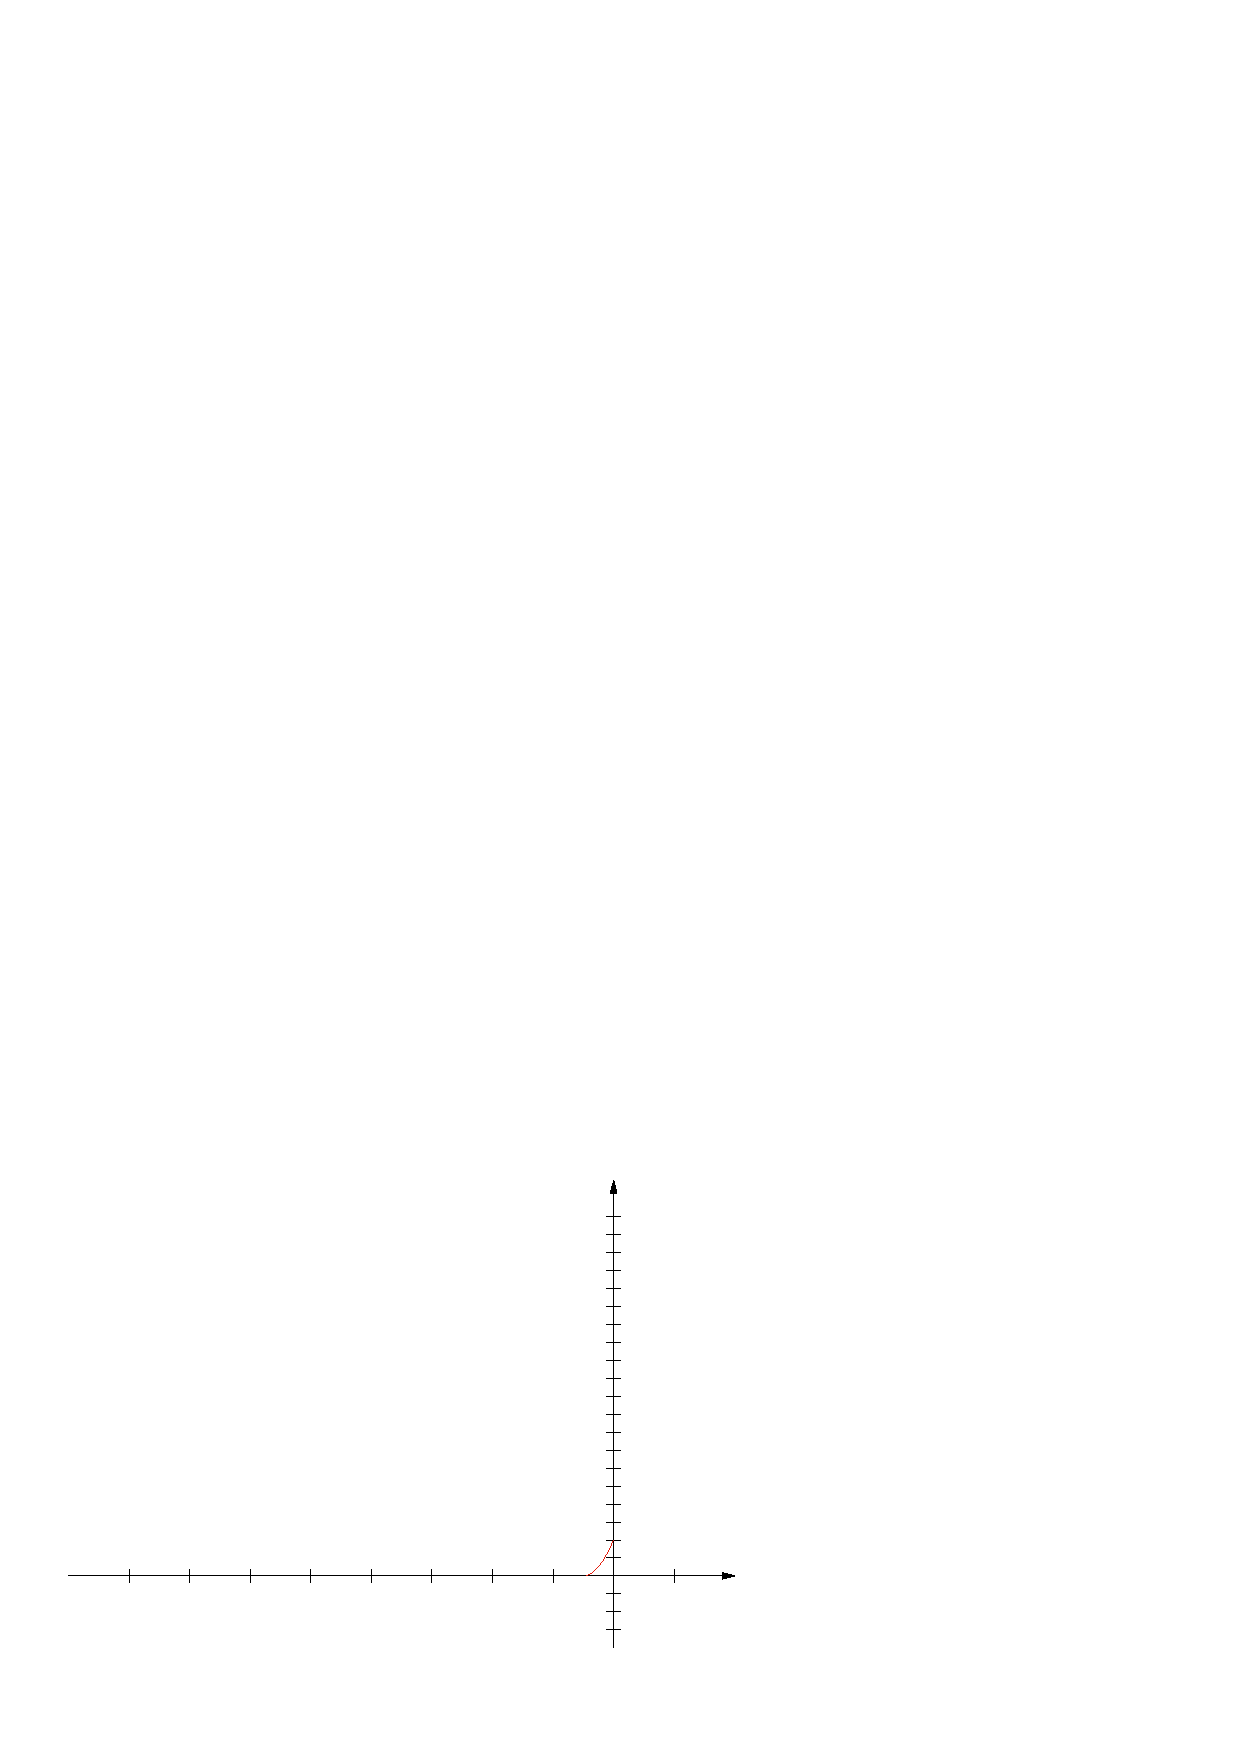
\includegraphics[width={288.00bp},height={216.00bp}]{curve1}}%
    \gplfronttext
  \end{picture}%
\endgroup

    \caption{Variación de la curva característica de transferencia.}
    \label{curve1}
\end{figure}

\section{Resistencias disponibles}
Se cuenta con una seria de resistencias de $0.5[\text{W}]$ con los valores
detallados en el \textbf{Cuadro~\ref{resistencias}}.

\begin{table}[!h]
\begin{center}
    \begin{tabular}{|c|c|c|c|c|c|c|c|c|c|}
    \hline
    $1[\Omega]$ & $10[\Omega]$ & $22[\Omega]$ & $47[\Omega]$ & $100[\Omega]$ &
    $150[\Omega]$ & $200[\Omega]$ & $220[\Omega]$ & $270[\Omega]$ &
    $330[\Omega]$
    \tabularnewline \hline
    $470[\Omega]$ & $510[\Omega]$ & $680[\Omega]$ & $1[k{\Omega}]$ &
    $2[k{\Omega}]$ & $2.2[k{\Omega}]$ & $3.3[k{\Omega}]$ & $4.7[k{\Omega}]$ &
    $5.1[k{\Omega}]$ & $6.8[k{\Omega}]$
    \tabularnewline \hline
    $10[k{\Omega}]$ & $20[k{\Omega}]$ & $47[k{\Omega}]$ & $51[k{\Omega}]$ &
    $68[k{\Omega}]$ & $100[k{\Omega}]$ & $220[k{\Omega}]$ & $330[k{\Omega}]$ &
    $510[k{\Omega}]$ & $1[M{\Omega}]$
    \tabularnewline \hline
    \end{tabular}
\end{center}
\caption{Resistencias disponibles para el calculo.}
\label{resistencias}
\end{table}

\section{Calculo de las resistencias}
Haciendo uso del software \emph{Octave} se calculan los valores de resistencias
que combinadas hallan el punto $Q$, y que han sido seleccionadas con las
siguientes condiciones:

\begin{equation*}
    \begin{split}
        V_{\text{GS}} \rightarrow 0.5\,V_{\text{GS(corte)}}\\
        I_{\text{D}} \rightarrow 0.5\,I_{\text{DSS}}\\
        0.02[\text{W}] < \{P_{R_1}, P_{R_2}, P_{R_D}, P_{R_S}\} < 0.16[\text{W}]\\
    \end{split}
\end{equation*}

\footnotesize
\begin{shaded}
\begin{verbatim}
% polarizacion por divisor de voltaje

Vdd = 9;            % [V]

Idss = 18.25e-3;    % [A]
Vgso = -1.129;      % [V]

% resistencias disponibles
R = [
    1 ...
    10 22 47 ...
    100 150 200 220 270 330 470 510 680 ...
    1000 2000 2200 3300 4700 5100 6800 ...
    10000 20000 47000 51000 68000 ...
    100000 220000 330000 510000 ...
    1000000
];

count = 1;
printf(
    '\tR1[Ω]\tR2[Ω]\tRd[Ω]\tRs[Ω]\t->
    \t\t\t\t\tVg[V]\tId[mA]\t\tP1[mW]\tP2[mW]\tPd[mW]\tPs[mW]\n'
);

for (h = 1:length(R))
    for (i = 1:length(R))
        for (j = 1:length(R))
            for (k = 1:length(R))
                R1 = R(h);
                R2 = R(i);
                Rd = R(j);
                Rs = R(k);

                Vg = (R2 / (R1 + R2)) * Vdd;    % Id = 0
                Id = Vg / Rs;                   % Vgs = 0

                _Vg = roots([
                    Idss/Vgso^2,
                    (1/Rs) - (2*(Idss/Vgso)),
                    Idss-Id
                ]);

                _Id = (1/Rs) * (Vg - _Vg(2));

                P1 = ((Vdd - Vg)^2) / R1;
                P2 = Vg^2 / R2;
                Pd = _Id^2 * Rd;
                Ps = _Id^2 * Rs;

                if(
                    (0.02<P1) && (P1<0.1) &&                     % 0.02 < P1 < 0.1
                    (0.02<P2) && (P2<0.1) &&                     % 0.02 < P2 < 0.1
                    (0.02<Pd) && (Pd<0.1) &&                     % 0.02 < Pd < 0.1
                    (0.02<Ps) && (Ps<0.1) &&                     % 0.02 < Ps < 0.1
                    (abs((0-_Vg(2)) - (_Vg(2)-Vgso)) < 0.01) &&  % Vg -> Vgs0/2
                    (abs((Idss-_Id) - (_Id-0)) < 0.01)           % Id -> Idss/2
                )
                    printf(
                        '%d\t%d\t%d\t%d\t%d\t->
                        \t\t(%.2f, 0)\t(0, %.3f)\t%.2f\t%.3f\t%.2f\t%.2f\t%.2f\t%.2f\n',
                        count,
                        R1, R2, Rd, Rs,
                        Vg,
                        Id * 1e3,
                        _Vg(2),
                        _Id * 1e3,
                        P1 * 1e3,
                        P2 * 1e3,
                        Pd * 1e3,
                        Ps * 1e3
                    );

                    count++;
                endif
            endfor
        endfor
    endfor
endfor

\end{verbatim}
\end{shaded}
\normalsize

La salida del programa detalla los valores de las cuatro resistencias ($R_1$,
$R_2$, $R_{\text{D}}$, $R_{\text{S}}$), el voltaje compuerta-fuente
($V_{\text{GS}}$), la corriente de drenaje ($I_{\text{D}}$), y las potencias
en cada unos de los resistores.

\footnotesize
\begin{shaded}
\begin{verbatim}
     R1[Ω] R2[Ω] Rd[Ω] Rs[Ω] ->                     Vg[V]  Id[mA]   P1[mW] P2[mW] Pd[mW] Ps[mW]
1    270   220   1000  1000  -> (4.04,0) (0,4.041)  -0.56  4.603    91.09  74.22  21.19  21.19
2    270   220   2000  1000  -> (4.04,0) (0,4.041)  -0.56  4.603    91.09  74.22  42.37  21.19
3    270   220   2200  1000  -> (4.04,0) (0,4.041)  -0.56  4.603    91.09  74.22  46.61  21.19
4    270   220   3300  1000  -> (4.04,0) (0,4.041)  -0.56  4.603    91.09  74.22  69.91  21.19
5    270   220   4700  1000  -> (4.04,0) (0,4.041)  -0.56  4.603    91.09  74.22  99.57  21.19
6    330   270   1000  1000  -> (4.05,0) (0,4.041)  -0.56  4.611    74.25  60.75  21.27  21.27
7    330   270   2000  1000  -> (4.05,0) (0,4.041)  -0.56  4.611    74.25  60.75  42.53  21.27
8    330   270   2200  1000  -> (4.05,0) (0,4.041)  -0.56  4.611    74.25  60.75  46.78  21.27
9    330   270   3300  1000  -> (4.05,0) (0,4.041)  -0.56  4.611    74.25  60.75  70.18  21.27
10   330   270   4700  1000  -> (4.05,0) (0,4.041)  -0.56  4.611    74.25  60.75  99.95  21.27
\end{verbatim}
\end{shaded}
\normalsize

\section{Simulación}
Se utilizó el software \emph{Quite Universal Circuit Simulator.} versión 23.3.1
para simular el circuito, este puede verse en la
\textbf{Figura~\ref{simulacion1}}.

\begin{figure}[!h]
\centering
\includegraphics[scale=1.0]{simulacion/2N3819.eps}
\caption{Simulación del circuito.}
\label{simulacion1}
\end{figure}

Los valores calculados en el simulador pueden verse en el
\textbf{Cuadro~\ref{simulacion2}}.

\begin{table}[!h]
\begin{center}
    \begin{tabular}{|c|c|c|c||c|c|c|c|}
    \hline
    $R_1[\Omega]$ & $R_2[\Omega]$ & $R_D[\Omega]$ & $R_S[\Omega]$ &
    $V_{\text{GS}}[V]$ &
    $I_{\text{D}}[m{A}]$
    \tabularnewline \hline \hline
    $270$ & $220$ & $  1k$ & $1k$ & $0.561$ & $3.01$ \tabularnewline \hline
    $270$ & $220$ & $  2k$ & $1k$ & $0.581$ & $2.44$ \tabularnewline \hline
    $270$ & $220$ & $2.2k$ & $1k$ & $0.585$ & $2.26$ \tabularnewline \hline
    $270$ & $220$ & $3.3k$ & $1k$ & $0.596$ & $1.61$ \tabularnewline \hline
    $270$ & $220$ & $4.7k$ & $1k$ & $0.601$ & $1.17$ \tabularnewline \hline
    $330$ & $270$ & $  1k$ & $1k$ & $0.561$ & $3.01$ \tabularnewline \hline
    $330$ & $270$ & $  2k$ & $1k$ & $0.580$ & $2.44$ \tabularnewline \hline
    $330$ & $270$ & $2.2k$ & $1k$ & $0.584$ & $2.27$ \tabularnewline \hline
    $330$ & $270$ & $3.3k$ & $1k$ & $0.595$ & $1.62$ \tabularnewline \hline
    $330$ & $270$ & $4.7k$ & $1k$ & $0.600$ & $1.18$ \tabularnewline \hline
    \end{tabular}
\end{center}
\caption{Valores obtenidos de la simulación.}
\label{simulacion2}
\end{table}

\section{Experimento}
El circuito armado puede verse en la \textbf{Figura~\ref{armado1}}, alimentado
por una fuente estable de $9[\text{V}]$.

\begin{figure}[!h]
\centering
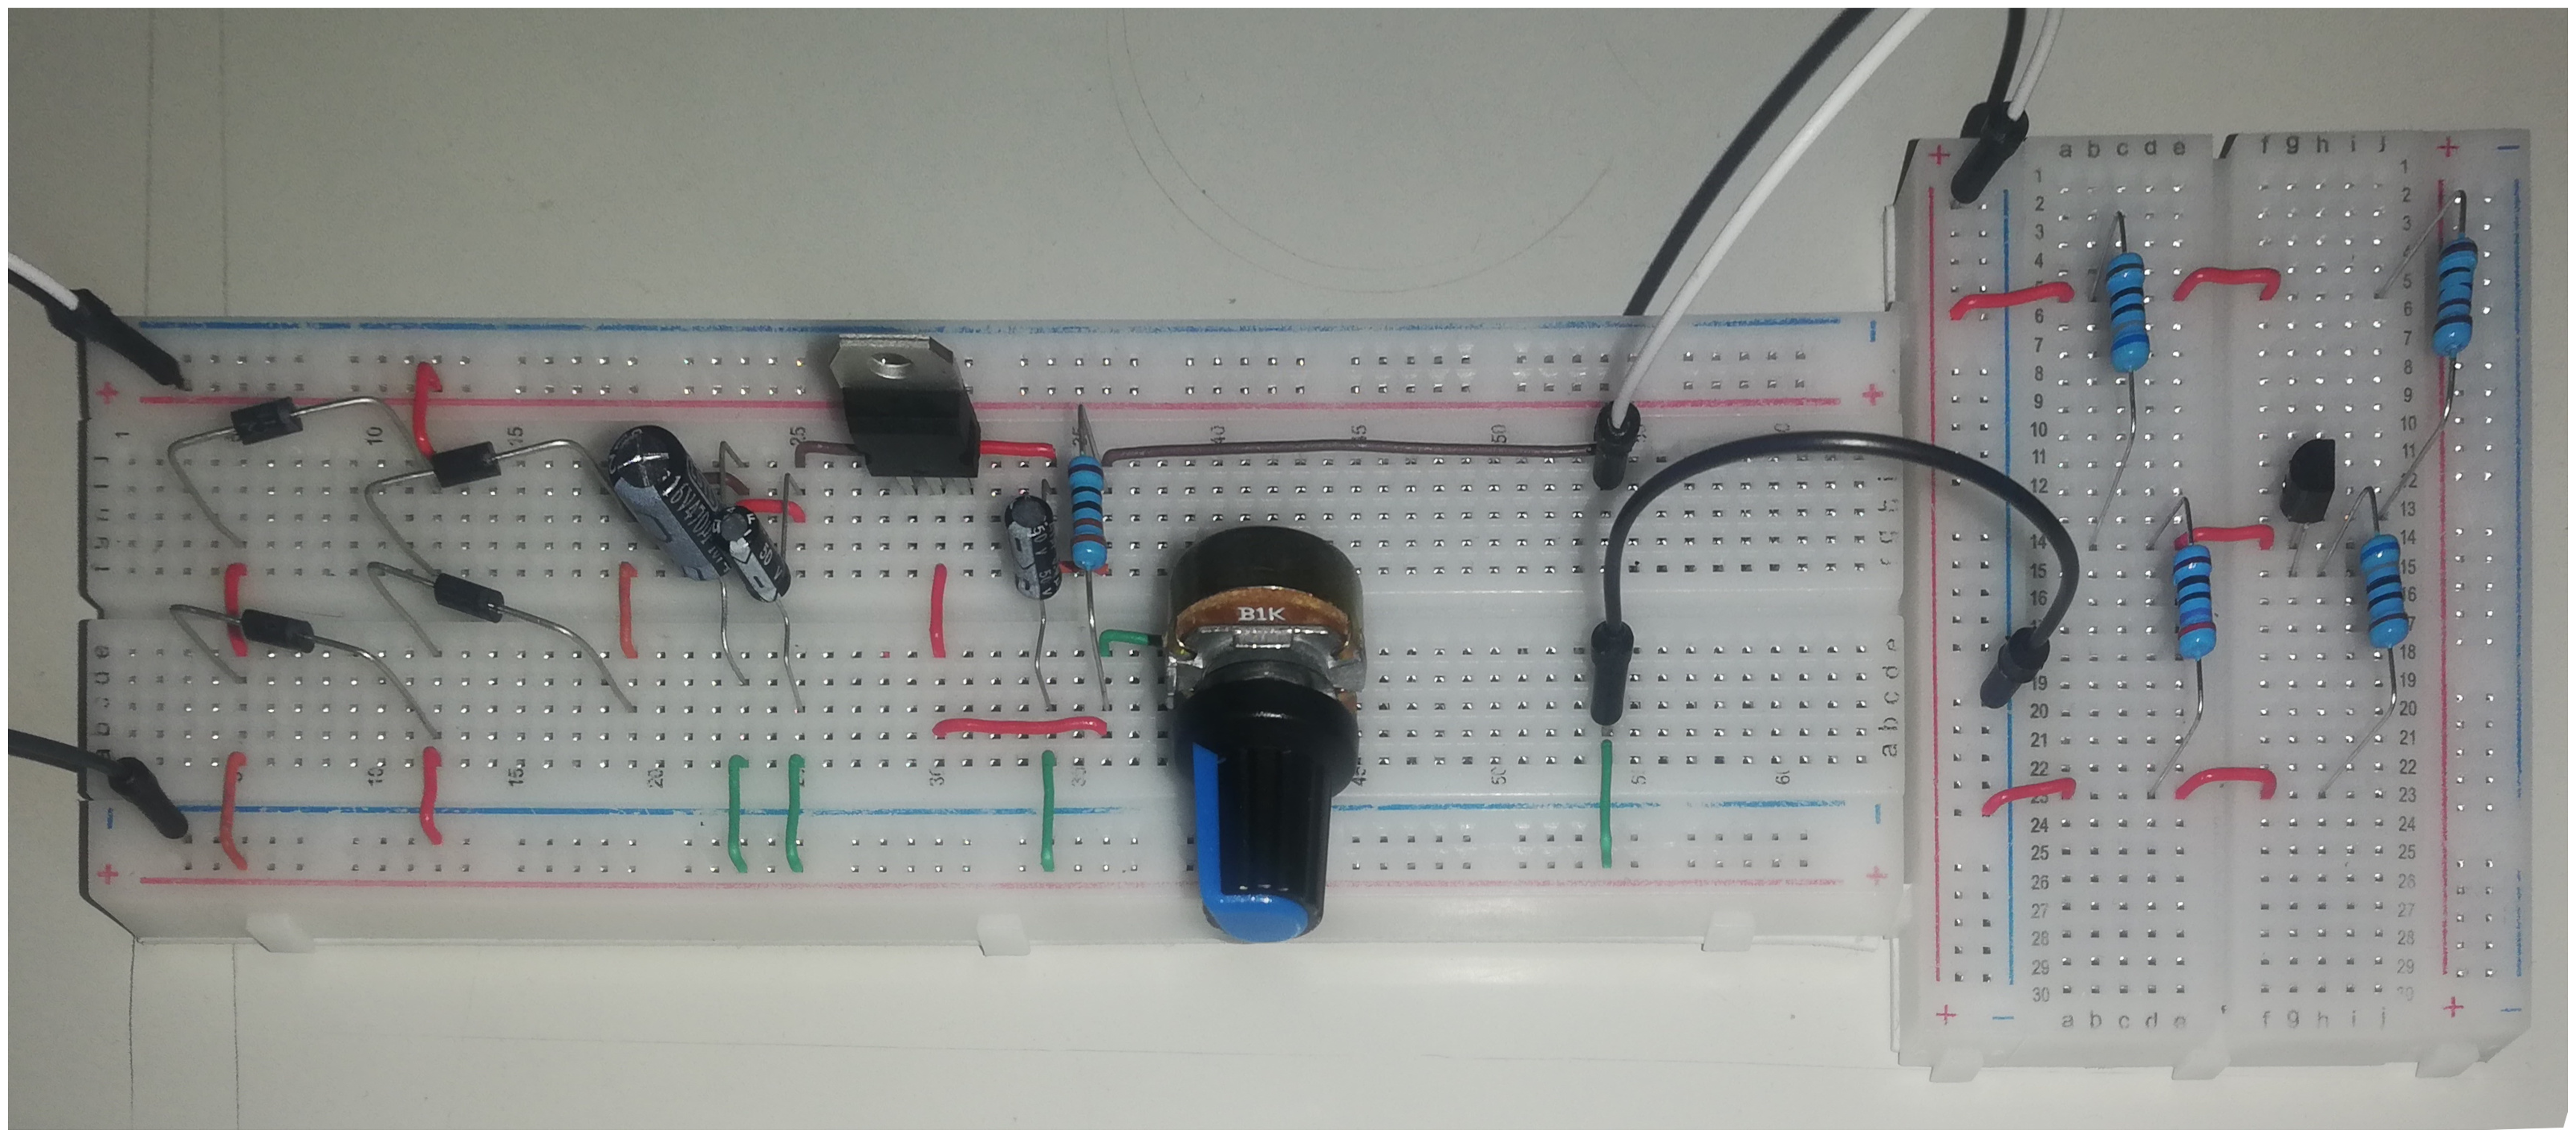
\includegraphics[scale=0.17]{fotos/circuito1.eps}
\caption{Circuito armado con una fuente de $9[\text{V}]$.}
\label{armado1}
\end{figure}

En el circuito se fueron variando las resistencias obtenidas, y se midieron los
valores de voltaje y corriente, estos se muestran en el
\textbf{Cuadro~\ref{armado2}}. Es notorio que en los cálculos teóricos los
valores de voltaje eran negativos, pero en la medición en el circuito la mayoría
son positivos. Así que se tomaran en cuenta únicamente los valores negativos.

\begin{table}[!h]
\begin{center}
    \begin{tabular}{|c|c|c|c||c|c|c|c|}
    \hline
    $R_1[\Omega]$ & $R_2[\Omega]$ & $R_D[\Omega]$ & $R_S[\Omega]$ &
    $V_{\text{GS}}[V]$ &
    $I_{\text{D}}[m{A}]$
    \tabularnewline \hline \hline
    $270$ & $220$ & $  1k$ & $1k$ & $-0.22$ & $4.28$ \tabularnewline \hline
    $270$ & $220$ & $  2k$ & $1k$ & $ 0.72$ & $2.84$ \tabularnewline \hline
    $270$ & $220$ & $2.2k$ & $1k$ & $ 0.79$ & $2.62$ \tabularnewline \hline
    $270$ & $220$ & $3.3k$ & $1k$ & $ 1.09$ & $1.85$ \tabularnewline \hline
    $270$ & $220$ & $4.7k$ & $1k$ & $ 1.27$ & $1.34$ \tabularnewline \hline
    $330$ & $270$ & $  1k$ & $1k$ & $-0.21$ & $4.29$ \tabularnewline \hline
    $330$ & $270$ & $  2k$ & $1k$ & $ 0.72$ & $2.83$ \tabularnewline \hline
    $330$ & $270$ & $2.2k$ & $1k$ & $ 0.79$ & $2.62$ \tabularnewline \hline
    $330$ & $270$ & $3.3k$ & $1k$ & $ 1.06$ & $1.84$ \tabularnewline \hline
    $330$ & $270$ & $4.7k$ & $1k$ & $ 1.26$ & $1.34$ \tabularnewline \hline
    \end{tabular}
\end{center}
\caption{Valores medidos en el circuito.}
\label{armado2}
\end{table}

\section{Conclusiones y recomendaciones}
El punto $Q$ hallado pueden apreciarse en la \textbf{Figura~\ref{curve2}}.
\begin{figure}[!h]
    \centering
    % GNUPLOT: LaTeX picture with Postscript
\begingroup
  \makeatletter
  \providecommand\color[2][]{%
    \GenericError{(gnuplot) \space\space\space\@spaces}{%
      Package color not loaded in conjunction with
      terminal option `colourtext'%
    }{See the gnuplot documentation for explanation.%
    }{Either use 'blacktext' in gnuplot or load the package
      color.sty in LaTeX.}%
    \renewcommand\color[2][]{}%
  }%
  \providecommand\includegraphics[2][]{%
    \GenericError{(gnuplot) \space\space\space\@spaces}{%
      Package graphicx or graphics not loaded%
    }{See the gnuplot documentation for explanation.%
    }{The gnuplot epslatex terminal needs graphicx.sty or graphics.sty.}%
    \renewcommand\includegraphics[2][]{}%
  }%
  \providecommand\rotatebox[2]{#2}%
  \@ifundefined{ifGPcolor}{%
    \newif\ifGPcolor
    \GPcolorfalse
  }{}%
  \@ifundefined{ifGPblacktext}{%
    \newif\ifGPblacktext
    \GPblacktexttrue
  }{}%
  % define a \g@addto@macro without @ in the name:
  \let\gplgaddtomacro\g@addto@macro
  % define empty templates for all commands taking text:
  \gdef\gplbacktext{}%
  \gdef\gplfronttext{}%
  \makeatother
  \ifGPblacktext
    % no textcolor at all
    \def\colorrgb#1{}%
    \def\colorgray#1{}%
  \else
    % gray or color?
    \ifGPcolor
      \def\colorrgb#1{\color[rgb]{#1}}%
      \def\colorgray#1{\color[gray]{#1}}%
      \expandafter\def\csname LTw\endcsname{\color{white}}%
      \expandafter\def\csname LTb\endcsname{\color{black}}%
      \expandafter\def\csname LTa\endcsname{\color{black}}%
      \expandafter\def\csname LT0\endcsname{\color[rgb]{1,0,0}}%
      \expandafter\def\csname LT1\endcsname{\color[rgb]{0,1,0}}%
      \expandafter\def\csname LT2\endcsname{\color[rgb]{0,0,1}}%
      \expandafter\def\csname LT3\endcsname{\color[rgb]{1,0,1}}%
      \expandafter\def\csname LT4\endcsname{\color[rgb]{0,1,1}}%
      \expandafter\def\csname LT5\endcsname{\color[rgb]{1,1,0}}%
      \expandafter\def\csname LT6\endcsname{\color[rgb]{0,0,0}}%
      \expandafter\def\csname LT7\endcsname{\color[rgb]{1,0.3,0}}%
      \expandafter\def\csname LT8\endcsname{\color[rgb]{0.5,0.5,0.5}}%
    \else
      % gray
      \def\colorrgb#1{\color{black}}%
      \def\colorgray#1{\color[gray]{#1}}%
      \expandafter\def\csname LTw\endcsname{\color{white}}%
      \expandafter\def\csname LTb\endcsname{\color{black}}%
      \expandafter\def\csname LTa\endcsname{\color{black}}%
      \expandafter\def\csname LT0\endcsname{\color{black}}%
      \expandafter\def\csname LT1\endcsname{\color{black}}%
      \expandafter\def\csname LT2\endcsname{\color{black}}%
      \expandafter\def\csname LT3\endcsname{\color{black}}%
      \expandafter\def\csname LT4\endcsname{\color{black}}%
      \expandafter\def\csname LT5\endcsname{\color{black}}%
      \expandafter\def\csname LT6\endcsname{\color{black}}%
      \expandafter\def\csname LT7\endcsname{\color{black}}%
      \expandafter\def\csname LT8\endcsname{\color{black}}%
    \fi
  \fi
    \setlength{\unitlength}{0.0500bp}%
    \ifx\gptboxheight\undefined%
      \newlength{\gptboxheight}%
      \newlength{\gptboxwidth}%
      \newsavebox{\gptboxtext}%
    \fi%
    \setlength{\fboxrule}{0.5pt}%
    \setlength{\fboxsep}{1pt}%
    \definecolor{tbcol}{rgb}{1,1,1}%
\begin{picture}(5760.00,5760.00)%
    \gplgaddtomacro\gplbacktext{%
      \csname LTb\endcsname%%
      \put(1571,160){\makebox(0,0)[r]{\strut{}}}%
      \put(1571,419){\makebox(0,0)[r]{\strut{}}}%
      \put(1571,678){\makebox(0,0)[r]{\strut{}}}%
      \put(1571,937){\makebox(0,0)[r]{\strut{}}}%
      \put(1571,1196){\makebox(0,0)[r]{\strut{}}}%
      \put(1571,1455){\makebox(0,0)[r]{\strut{}}}%
      \put(1571,1714){\makebox(0,0)[r]{\strut{}}}%
      \put(1571,1973){\makebox(0,0)[r]{\strut{}}}%
      \put(1571,2232){\makebox(0,0)[r]{\strut{}}}%
      \put(1571,2491){\makebox(0,0)[r]{\strut{}}}%
      \put(1571,2750){\makebox(0,0)[r]{\strut{}}}%
      \put(1571,3009){\makebox(0,0)[r]{\strut{}}}%
      \put(1571,3268){\makebox(0,0)[r]{\strut{}}}%
      \put(1571,3527){\makebox(0,0)[r]{\strut{}}}%
      \put(1571,3786){\makebox(0,0)[r]{\strut{}}}%
      \put(1571,4045){\makebox(0,0)[r]{\strut{}}}%
      \put(1571,4304){\makebox(0,0)[r]{\strut{}}}%
      \put(1571,4563){\makebox(0,0)[r]{\strut{}}}%
      \put(1571,4822){\makebox(0,0)[r]{\strut{}}}%
      \put(1571,5081){\makebox(0,0)[r]{\strut{}}}%
      \put(1571,5340){\makebox(0,0)[r]{\strut{}}}%
      \put(1571,5599){\makebox(0,0)[r]{\strut{}}}%
      \put(716,196){\makebox(0,0){\strut{}}}%
      \put(1667,196){\makebox(0,0){\strut{}}}%
      \put(2618,196){\makebox(0,0){\strut{}}}%
      \put(3569,196){\makebox(0,0){\strut{}}}%
      \put(4520,196){\makebox(0,0){\strut{}}}%
      \put(5471,196){\makebox(0,0){\strut{}}}%
      \csname LTb\endcsname%%
      \put(6422,134){\makebox(0,0)[l]{\strut{}$V_{\text{GS}}[V]$}}%
      \put(1857,5858){\makebox(0,0)[l]{\strut{}$I_{\text{D}}[mA]$}}%
      \put(50,134){\makebox(0,0)[l]{\strut{}$-1.129$}}%
      \put(887,134){\makebox(0,0)[l]{\strut{}$-0.56$}}%
      \put(5376,134){\makebox(0,0)[l]{\strut{}$4.041$}}%
      \put(1904,5146){\makebox(0,0)[l]{\strut{}$18.25$}}%
      \put(1904,1610){\makebox(0,0)[l]{\strut{}$4.603$}}%
    }%
    \gplgaddtomacro\gplfronttext{%
    }%
    \gplgaddtomacro\gplbacktext{%
      \csname LTb\endcsname%%
      \put(1571,160){\makebox(0,0)[r]{\strut{}}}%
      \put(1571,419){\makebox(0,0)[r]{\strut{}}}%
      \put(1571,678){\makebox(0,0)[r]{\strut{}}}%
      \put(1571,937){\makebox(0,0)[r]{\strut{}}}%
      \put(1571,1196){\makebox(0,0)[r]{\strut{}}}%
      \put(1571,1455){\makebox(0,0)[r]{\strut{}}}%
      \put(1571,1714){\makebox(0,0)[r]{\strut{}}}%
      \put(1571,1973){\makebox(0,0)[r]{\strut{}}}%
      \put(1571,2232){\makebox(0,0)[r]{\strut{}}}%
      \put(1571,2491){\makebox(0,0)[r]{\strut{}}}%
      \put(1571,2750){\makebox(0,0)[r]{\strut{}}}%
      \put(1571,3009){\makebox(0,0)[r]{\strut{}}}%
      \put(1571,3268){\makebox(0,0)[r]{\strut{}}}%
      \put(1571,3527){\makebox(0,0)[r]{\strut{}}}%
      \put(1571,3786){\makebox(0,0)[r]{\strut{}}}%
      \put(1571,4045){\makebox(0,0)[r]{\strut{}}}%
      \put(1571,4304){\makebox(0,0)[r]{\strut{}}}%
      \put(1571,4563){\makebox(0,0)[r]{\strut{}}}%
      \put(1571,4822){\makebox(0,0)[r]{\strut{}}}%
      \put(1571,5081){\makebox(0,0)[r]{\strut{}}}%
      \put(1571,5340){\makebox(0,0)[r]{\strut{}}}%
      \put(1571,5599){\makebox(0,0)[r]{\strut{}}}%
      \put(716,196){\makebox(0,0){\strut{}}}%
      \put(1667,196){\makebox(0,0){\strut{}}}%
      \put(2618,196){\makebox(0,0){\strut{}}}%
      \put(3569,196){\makebox(0,0){\strut{}}}%
      \put(4520,196){\makebox(0,0){\strut{}}}%
      \put(5471,196){\makebox(0,0){\strut{}}}%
      \csname LTb\endcsname%%
      \put(6422,134){\makebox(0,0)[l]{\strut{}$V_{\text{GS}}[V]$}}%
      \put(1857,5858){\makebox(0,0)[l]{\strut{}$I_{\text{D}}[mA]$}}%
      \put(50,134){\makebox(0,0)[l]{\strut{}$-1.129$}}%
      \put(887,134){\makebox(0,0)[l]{\strut{}$-0.56$}}%
      \put(5376,134){\makebox(0,0)[l]{\strut{}$4.041$}}%
      \put(1904,5146){\makebox(0,0)[l]{\strut{}$18.25$}}%
      \put(1904,1610){\makebox(0,0)[l]{\strut{}$4.603$}}%
    }%
    \gplgaddtomacro\gplfronttext{%
    }%
    \gplbacktext
    \put(0,0){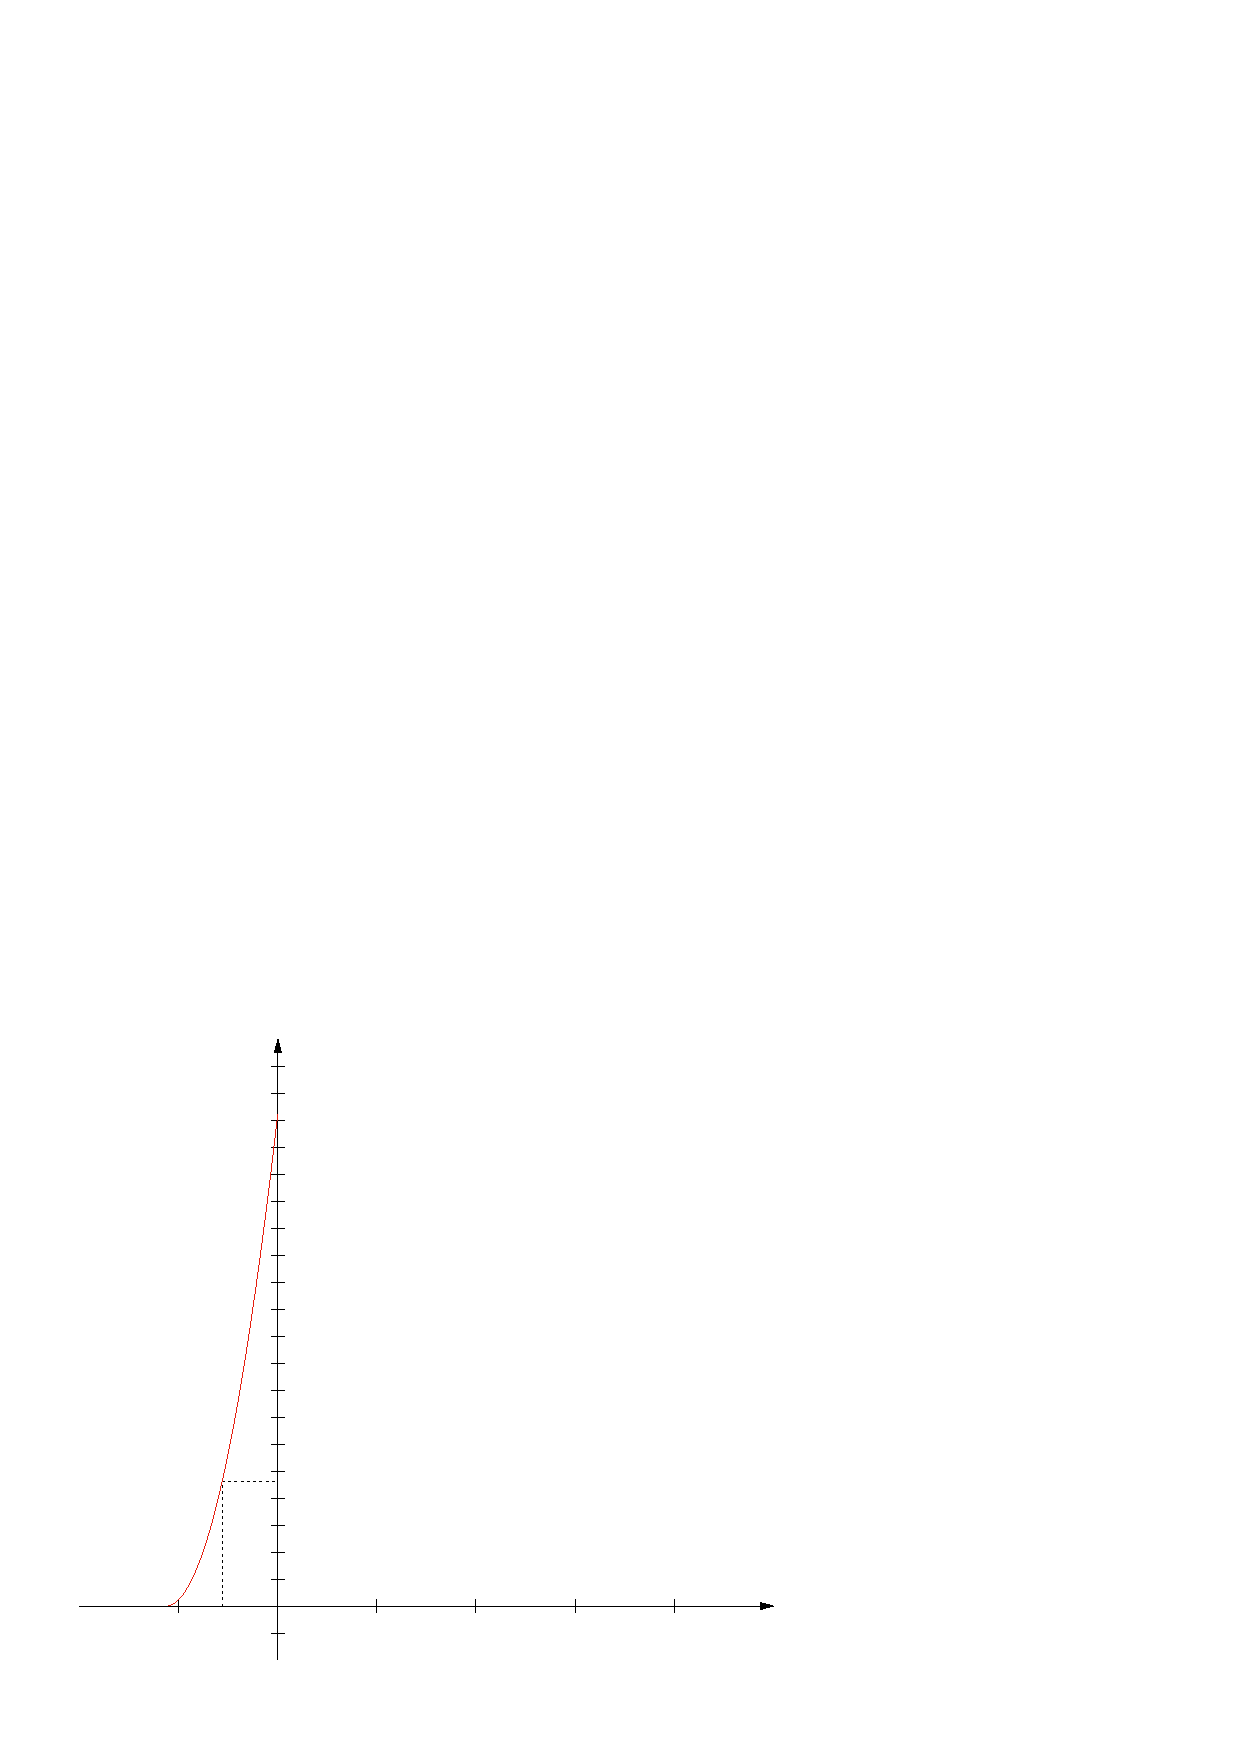
\includegraphics[width={288.00bp},height={288.00bp}]{curve2}}%
    \gplfronttext
  \end{picture}%
\endgroup

    \caption{Punto $Q$ hallado.}
    \label{curve2}
\end{figure}

\begin{equation*}
    \begin{split}
        R_1 &= 270[\Omega]\\
        R_2 &= 220[\Omega]\\
        R_D &= 1k[\Omega]\\
        R_S &= 1k[\Omega]\\
    \end{split}
\end{equation*}

\begin{thebibliography}{99}

\bibitem{Floyd}
Thomas L. Floyd (2008).\\
\textbf{Dispositivos electrónicos. 8va Edición.}\\
Pearson Education\\

\bibitem{2N3819} \textbf{2N3819 N-Channel RF Amplifier.}\\
Extraído el 11 de Noviembre del 2024, de: \\
\url{https://www.alldatasheet.com/datasheet-pdf/view/171937/FAIRCHILD/2N3819.html}.

\end{thebibliography}

\end{document}

